\chapter{Word2Vec}

In dieser Kapitel wird das Verfahren "Word2Vec" durch die Nutzung von Neuronalem Netz vorgestellt. Word2Vec ist eine Darstellung von Wörtern mit Vecoren, was auch aus die Abkürzung klar wird - Word ist klar; 2 - to; und Vec - Vector und das ganze "word to vector". Dieses Model ist am meisten  in der Natural Laguage Processing (NLP) verbreitet und wird in vielen Bereichen der Informatik genutzt, unter anderem in Spamfilterung und Dokumentenanalyse. Jedoch diese Technik besagt nur wie die Wörter eines Textes dargestellen werden können. Das Verfahren, bei dem die möglichst passenden Vektoren in einem ausgewählten Text, auch Corpus genant, gelernt werden, heißt Word Embeddings. Bei dieser Technik wird ein Neuronales Netzt eigesetzt. Die Vorgehensweise und die Idee wird folglich erklärt.

\section{Word Embedding}

Wie es schon in der Einleitung erwähnt wurde, Word Embedding ist der Prozess, bei dem die Wörter eines Textes in mathematischen Vektoren gewandelt werden. Zuerst muss der Corpus vorbeiretet werden. Ich stelle hier nur die Theorie und in einer späteren Kapitel (!? WICHTIG WELCHE GENAU!?) gehe ich tiefer in dem Programmcode.

\!!! DAS HIER GEHÖRT IN EINE ANDERE KAPITEL !!!
!!! DIE KAPITEL FÜR TEXTVORBEREITUNG ODER SOWAS!!!

Als der Text vorbeitet ist, sodass es von Sonderzeichen und alle unnötigen Zeichen bereinigt wird. Wenn der Text vorbeireitet ist, werden die Wörter aus dem Corpus bestimmt und jeder erhält einen Index. Üblicherweise werden die Wörter nach ihrer Häufigkeit angeordnet. Das häufigste Wort erhält somit den Index 1. Als nächstes werden die Wörter im Korpus durch ihren Index ersetzt, um alle Trainingspaare fürs Lernen generiert zu werden. Dies erfolgt in dem es durch das Corpus iteriert und in einem bestimmten Fenster, oder in der Literatur auch als Window gezeichnet, alle Contextwörter und den Targetwort ausgelesen werden. Das Targetwort ist das Wort in der Mitte, während die Wörter um das Targetwort entsprechend die Kontextwörter. 

!!! BIS HIER MUSS WEG !!!!

In der Literatur werden zwei Arten von Wort2Vec Modelle - SKIP-gram und CBOW (Continous Bag of Words). Beide Modelle verwenden ein Neuronales Netz mit einem oder zwei versteckten Schichten (siehe !!KAPITEL MIT DEM PROGRAMMCODE!!). Die beiden Methoden unterscheiden sich nach ihren Ein- und Ausgaben.   

\subsubsection{SKIP-gram Model}
Bei dem SKIP-gram-Model fließen die Targetwörter als Eingabe und das Model versucht ein Kontextwort zu raten. Hier ist die Struktur eines Skip-gram Models:

\begin{figure}
	\centering
	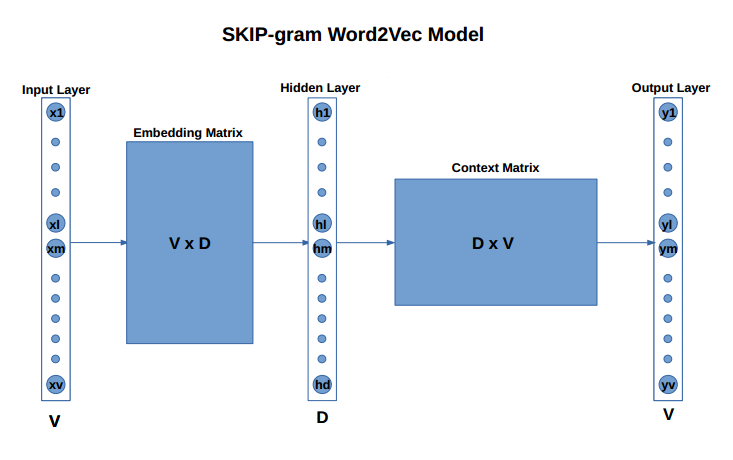
\includegraphics[scale=0.5]{images/SKIP_Model.png}
	\caption{Skip-gram Word2Vec Model}
	\label{skip}
\end{figure}

Aus der Abbildung \ref{skip} ist es zu entnehmen, dass ein Skip-gram Model aus einer hidden Schicht und zwei Eigabeschichten. Die Eingabe sowie die Ausgabe ist ein Vektor, der aus $\emph{V}$ Componente besteht. Das entspricht die größe des Wörterbuchs (engl. Vocabulary). Das versteckte Schicht besteht aus $\emph{D}$ Variablen und stellt einen Vektor dar. Die Dimensionalität dieses Vektors nimmt üblich einen Wert zwischen 25 und 300. Diese Variablen können auch als Eigenschaften für die Wörter betrachtet werden. Je mehr Kriterien es untersucht werden, desto besser die Beziehung zwischen Wörtern wiederspiegelt werden kann. Die Ausgabe ist wieder einen $\emph{V-dimensionalen}$ Vektor. Jedoch die Ausgabe ist kein One-Hot Vektor mehr, der das Kontextwort wiedergibt, sondern einen Wahrscheinlichkeitsvektor, dass der Wort mit der entsprechenden Index der richtige Contextwort ist.

Die zwei Matrizen sind identisch, jedoch die Kontextmatrize ist die transponierte Embeddingsmatrize. Diese Matrix beinhaltet unsere Wortvektoren.

Der Abbildung \ref{skip} nach besteht das neuronale Netz aus drei Schichten. Im Hiddenlayer steht ein Vektor, der abhängig von unsere Eingabe den Wortvektor repräsentiert. Die Ausgabe ist ein softmax

\subsubsection{CBOW Model}
Die Kontextwörter sind die Eingabe in dem CBOW-Model und das Model ratet der Targetwort. Die zwei Modelle besitzen die gleiche Anzahl an Schichten. Das CBOW-Model ist ein umgedrehtes SKIP-gram-Model, jedoch die Eingabe besteht aus $\emph{w}$-Viele Vektoren statt nur eins. Als nächstes stellt die \ref{cbow} Abbildung die beschriebene Struktur.

\begin{figure}
	\centering
	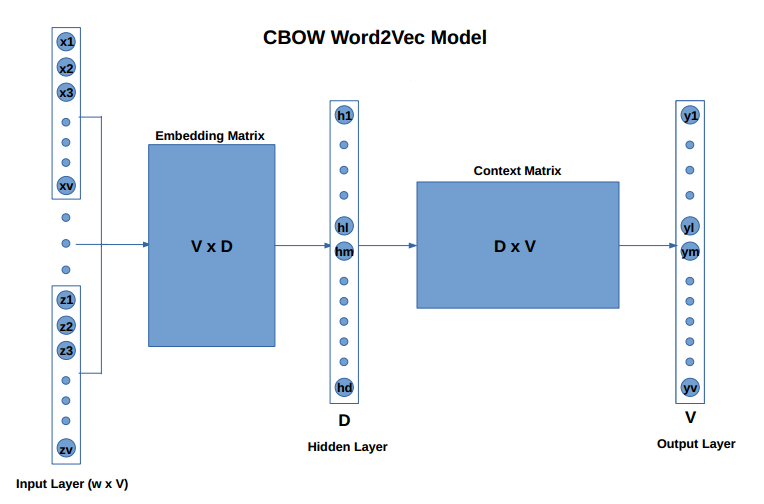
\includegraphics[scale=0.5]{images/CBOW_Model.png}
	\caption{CBOW Word2Vec Model}
	\label{cbow}
\end{figure}

Die Struktur des CBOW-Models besteht wieder aus eine Matrix für das Embedding der Target- und Kontextwörter. Die größe der Matrizen hängt von der ausgewählten Hyperparameter und die Größe des Datensatzes. Die Anzahl der verwendeten Inputvektoren entspricht die größe des gesetzten Window (Kontextfenster).

\subsection{Implementierung}